
\section{Manual Obfuscation in Modeling Assignments}\label{sec:human-plagiarism}
% --------------------------
% Related Work / Gap
% --------------------------
How students plagiarize programming assignments and which ways they employ to obfuscate their plagiarism is well researched \cite{Novak2019}.
This includes classifications of code obfuscation techniques \cite{Faidhi1987, Karnalim2016} and the automated detection of plagiarism in student submissions \cite{prechelt2002}.
However, as discussed in \autoref{sec:mde-challenges}, only limited research exists on plagiarism in modeling assignments. Furthermore, modeling assignments are susceptible to plagiarism since they are complex and require domain understanding and problem-solving skills \cite{Martinez2020}.
Yet, these assignments are often the only way to evaluate the student's performance~\cite{Ciccozzi2018}.
How students engage in plagiaristic behaviors in modeling assignments remains unclear.
Related work from the domain of modeling clone detection \cite{Babur2019} does not address this issue: Plagiarism detection involves an attacker scenario, where the plagiarizer intentionally tries to conceal the plagiarism by employing various obfuscation techniques. In contrast, clone detection focuses on identifying identical or similar sections in models without considering deliberate obfuscation by plagiarizers.
Therefore, the insights from modeling clone detection cannot be directly applied to the context of modeling plagiarism.
In essence, the lack of knowledge about students' plagiaristic behaviors hinders detection efforts.

% --------------------------
% Contribution
% --------------------------
We address this gap by systematically analyzing how students plagiarize and obfuscate in modeling assignments.
We present the results of an experiment where ten novice modelers were asked to plagiarize a given metamodeling assignment's solution and conceal their plagiarism, i.e., hiding the relation to the original.
The experiment was conducted in a master-level practical modeling course, where each student was given 30 minutes to conceal the plagiarism in their solution copy.
We employed a mixed-method approach, combining quantitative analysis of the plagiarized metamodels and qualitative data from the participants' descriptions of how they tried to conceal the plagiarism.
We show how frequently different techniques were employed and to what level the models were altered.
In the experiment's result evaluation, we asked the course instructors to inspect both plagiarized and original solutions.
Additionally, we applied a state-of-the-art plagiarism detector~\cite{Saglam2022} to test the automatic plagiarism detection quality.
With this experiment, we set out to answer the following key questions:

\begin{enumerate}%[style=unboxed,leftmargin=0cm,topsep=3pt]
    \item How do novice modelers conceal modeling plagiarism?
    \item Can their modeling plagiarism be detected by the instructors?
    \item Can their modeling plagiarism be detected by plagiarism detectors?
\end{enumerate}

\noindent
The experiment shows how the ten participants engage in modeling plagiarism and how they describe their approach.
%
The results show that the participants employ various obfuscation techniques, with the renaming of elements occurring most frequently, followed by reordering elements.
On average, students alter every second element of the modeling assignment. Nevertheless, human and tool-based inspection can still detect these instances of plagiarism.
However, manual inspection quickly becomes impractical with large course sizes.
This paper contributes to a better understanding of plagiarism in modeling assignments by investigating students' obfuscation techniques.
Ultimately, we provide insights to enhance fairness and academic integrity in assessing modeling assignments.

\subsection{Experiment Design}\label{sec:human-plagiarism-task}
%\todo{slide figure about the process: original --> student --> plag + descr}

\noindent
We conducted an experiment with novice modelers, where they plagiarized an \ac{EMF} metamodel and obfuscated the relation to the original metamodel.
In total, ten students voluntarily participated in the experiment.
%
The experiment consisted of two tasks conducted sequentially.
First, the participants were asked to copy and modify a given source metamodel to conceal the plagiarism while still fulfilling the given assignment.
Second, we asked the participants for a brief description outlining their techniques to disguise the act of plagiarism and its relation to the original solution.
%
We employed a mixed-method approach, combining quantitative analysis of the plagiarized metamodels and qualitative data from the participants' descriptions of how they tried to conceal the plagiarism. 
%
The duration of the experiment was 30 minutes. 
Since participants used their own solutions as a basis for plagiarism, they did not require additional familiarization with the solution. For an experiment where the participants are unfamiliar with the given solution, a larger time frame would have been required.

\textbf{Scenario:}
We instructed the participants to imagine a scenario where a deadline for a modeling assignment was coming up. However, they had access to a solution provided by a hypothetical classmate and thus decided to plagiarize it. To that end, the participants were asked to conceal the plagiarism from the instructor of the hypothetical course while still fulfilling the assignment.
In detail, we gave the following instructions regarding the obfuscation:

\begin{myquote}
\textit{1. Create a copy of the metamodel.}
    
\textit{2. Modify the copy to disguise the plagiarism (the examiner will only assess the metamodel).}
    
\textit{3. Make sure that the modifications have been saved.}
\end{myquote}

Finally, we asked them to describe how they proceeded during the task and what types of modifications they used.

\textbf{Participants:}
We conducted our experiment with ten students from a practical course on model-driven software development.
It is a master's level computer science elective course at Karlsruhe Institute of Technology, Germany. 
The students are novice practitioners of model-driven engineering and had little to no prior metamodeling experience before attending the course. They have basic knowledge of \ac{UML} diagrams and object-oriented modeling.
The course covers typical~\cite{Ciccozzi2018} topics like (meta)modeling and model transformations.
They participated in the experiment after completing the course's metamodeling assignment.

\textbf{Metamodeling Assignment:}
Our experiment uses a typical~\cite{Ciccozzi2018} modeling assignment~\cite{Saglam2023_supp} of an \ac{MDE} practical course (master's level elective course, no prior metamodeling experience), which tasks the students with creating an \ac{EMF} metamodel for designing component-based system architectures. The metamodel includes four different architectural views: The component repository, the component assembly, the system's hardware environment, and the components' allocation.
The task is loosely inspired by the Palladio component model~(PCM)~\cite{reussner2016a}.
%
The \textit{repository} manages all components and interfaces that may be reused within multiple systems. The \textit{assembly} shows how components are instantiated and interconnected. The \textit{environment} depicts all containers and their links. The \textit{allocation} specifies which components are allocated on which containers of the environment.
%
The goal of the assignment is to design an \ac{EMF} metamodel that allows modeling systems such as the media store architecture in \autoref{fig:mediastore}.
%
Students usually solve this modeling assignment in groups, ranging between two and five students. 
In the past, students' solutions for this assignment contained, on average, five packages, 39 classifiers, 45 references, ten attributes, and one operation \cite{Saglam2022}.
Most metamodels were designed in a single file, but some students fragmented them into up to 7 files.

\begin{figure}
    \centering
    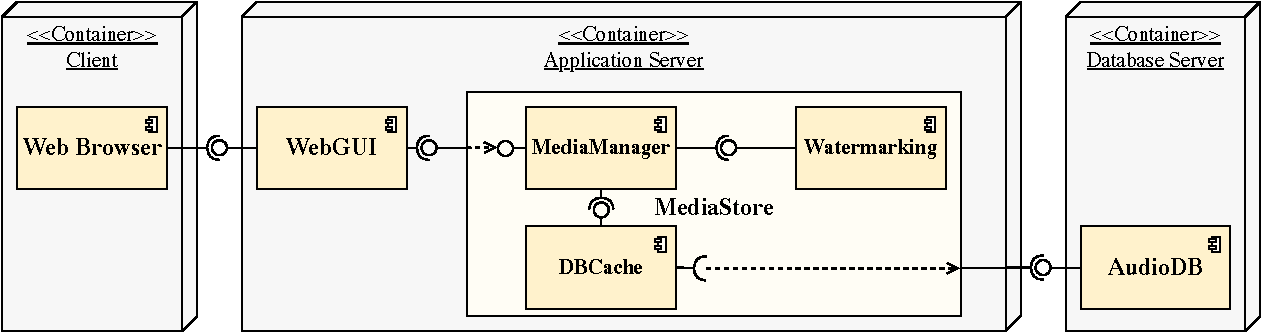
\includegraphics[width=0.99\linewidth]{figures/mediastore.pdf}
    \caption[Example Instance for the Modeling Assignment]{Component-based architecture of a media store, which the assignment's metamodel should be able to represent. Loosely based on the work of \citet{becker2008a}.}
    \label{fig:mediastore}
\end{figure} 

\textbf{Ethical Considerations:}
During this experiment, ethical considerations were given due attention. Participants voluntarily partook and were fully informed about the experiment's scope and purpose. They explicitly agreed to use and publish their artifacts for research purposes, ensuring confidentiality by anonymizing them.% Transparency and respect for participants were principles upheld during the study.

\subsection{Observed Results}
%\todo{(LOW) Examples aus Vortrag zu Figures machen.}


%\citet{Babur2019}:
%\begin{description}[style=unboxed,leftmargin=5pt]
%    \item[Type-A] Exact duplicates except for layout, formatting, internal ids, and cosmetic name changes (lower-/uppercase)
%    \item[Type-B] Duplicates with smaller syntactic/semantic changes to names, types, attributes, and minor additions/removals.
%    \item[Type-C] Duplicate larger changes/additions/removals of elements, names, types, and attributes.
%    \item[Type-D] Semantically duplicates with different structures and content.
%\end{description}

%\citet{Faidhi1987,Karnalim2016}:
%\begin{description}[style=unboxed,leftmargin=5pt]
%    \item[Level 0:] Verbatim copy.
%    \item[Level 1:] Changes in comments and indentation.
%    \item[Level 2:] Changes in names.
%    \item[Level 2.5:] Changes to packages and package namespaces (introduced by \cite{Karnalim2016}).
%    \item[Level 3:] Changes in declarations (e.g., adding extra constants, changing the positions of declared variables, shuffling the methods, etc.).
%    \item[Level 4:] Changes in pro wordgram modules (e.g., encapsulating statements in methods, using either parameters or global variables, inserting dummy methods).
%    \item[Level 5:] Changes in program statements (e.g., using FOR instead of WHILE, etc.).
%    \item[Level 6:] Changes in the decision logic (e.g., changes in expressions, loops to recursion, rearranging loosely coupled statements).
%\end{description}

\begin{table*}[t]
	\centering
    \small
	\begin{tabular}{l p{215pt} r r r} % nach letztem c @{\hskip 2em}
		\toprule
		Techniques         & Description                                                                       & \footnotesize\#Occ. & \footnotesize\#Part. & \footnotesize Type\\
		\midrule
		Cosmetic Renaming  & Changing capitalization of names, introducing or resolving typographical errors.                 & 1    & 1    & A                     \\
		Minor Renaming     & Introducing or resolving abbreviations, adding and removing suffixes or prefixes. & 85   & 9    & B                     \\
		Major Renaming     & Changing names to synonyms, translations, or entirely different names.            & 141  & 7    & C                     \\
		\midrule
		Reorder Features  & Re-ordering attributes and references of a classifier.                            & 10   & 1    & B                     \\
		Reorder Package   & Re-ordering the model elements contained within a single package.                       & 57   & 4    & B                     \\
		Reorder Classifiers & Moving classifiers from one package to another (re-ordering across the model).  & 1    & 1    & C                     \\
		\midrule
		Introduce Package  & Create a package and add existing elements from other packages or other packages. & 20   & 3    & C                     \\
		Dissolve Package   & Deleting a package and moving its contained elements to other packages.           & 8    & 4    & C                     \\
		\midrule
		Delete Feature     & Delete an existing attribute, relation, or operation of a classifier.             & 26   & 7    & B                     \\
		Delete Classifier  & Delete an existing classifier from the model.                                     & 11   & 6    & C                     \\
		Delete Package     & Delete an existing package from the model (can be part of dissolving a package).  & 5    & 4    & B                     \\
		\midrule
        Insert Feature     & Insert a new attribute, relation, or operation into a classifier.                 & 6    & 4    & B                     \\
		Insert Classifier  & Insert a new classifier into the model.                                           & 10   & 3    & C                     \\
		Insert Package     & Inserting a new package into the model (may be combined with moving elements).    & 5    & 4    & B                     \\
		\midrule
        Change Property    & Changing an element's property, e.g., \textit{abstract} for classifiers, \textit{ordered} or the cardinality for references. & 31    & 3    & B                     \\
		\midrule
		Remove Inheritance & Remove inheritance relation between the two classifiers.                          & 4    & 1    & C                     \\
        Add Inheritance    & Add inheritance relation between the two classifiers.                             & 7    & 2    & C                     \\
		Change Inheritance & Changing the inheritance hierarchy structurally without changing it semantically. & 9    & 2    & D                     \\
		\bottomrule
	\end{tabular}
    \caption[Obfuscation Techniques by Novice Modelers]{Overview of the obfuscation techniques employed by the participants, classified according to \citet{Babur2019}. We include how often each technique occurred across all participants (denoted as \textit{\#Occ}) and how many participants employed it (denoted as \textit{\#Part}).}
	\label{tab:student-obfuscation}
%\todo{Do we want the midrules? And if yes how to we want to separate? e.g. for property?}
\end{table*}



\noindent
%
In this section, we present our findings~\cite{Saglam2023_supp}, analyze the participants' obfuscation techniques, examine human plagiarism detection effectiveness, and evaluate an automated tool's detection performance.

\paragraph{Obfuscation Techniques}
To analyze the obfuscation techniques employed by the students, we first used \textit{EMF Compare} to identify potential differences between the plagiarized models and their originals. Unsurprisingly, in some cases, EMF Compare did not accurately produce the correct differences~\cite{Wittler2023}, highlighting the limitation of relying solely on model differencing for plagiarism detection.
In the second step, we thus manually inspected the models, carefully examining them for potential obfuscation. To ensure the validity of our observations, we cross-referenced our findings with the textual descriptions provided by the students.
 %
In our experiment, the participants engaged in a range of individual alterations to obfuscate the plagiarism, with the number of alterations varying between 10 and 91. Thereby, we count semantic alterations, e.g., moving an element as a single one. The mean number of alterations is 43.7, while the median is 31.5. These results imply an average of approximately one alteration for every two model elements in the source model.

We classify the participant's techniques according to the modeling clone types from \citet{Babur2019}, based on the \ac{UML} clone types of \cite{Stoerrle2015}.
While designed for clones rather than plagiarism, this classification enables systematic categorization of plagiarism techniques.
\citet{Babur2019} describe \textbf{Type-A} clones as exact duplicates except for layout, formatting, internal IDs, and purely cosmetic name changes.
\textbf{Type-B} clones have minor syntactic and semantic changes to names, types, attributes, and minor additions or removals.
\textbf{Type-C} clones include more extensive alterations, additions, and removals of elements and their properties.
Finally, \textbf{Type-D} clones are semantically equivalent with different structures and content.

We provide an overview of the techniques, indicating the frequency of their application and the number of participants who utilized each technique.
%
As summarized in \autoref{tab:jplag-student-obf}, the participants employed various obfuscation methods during the experiment. The types of changes can be described as follows:
The most common method was renaming, accounting for about half of the total changes made by all participants. Notably, the participants tended to utilize sophisticated renaming strategies, resulting in the majority of these alterations being categorized as \textit{major renaming} and none as \textit{cosmetic renaming}. 
As an example of such major renaming, one participant renamed a classifier from \textit{"Component"} to \textit{"BuildingBlock"}.
%
Other properties, such as \textit{abstract} or \textit{ordered}, were also subject to changes, albeit less frequently than names.

Another common practice observed was the reordering of elements. However, most participants refrained from moving classifiers across packages. Instead, they focused on rearranging the contents of the packages themselves or altering the order of features within the classifiers. Some participants also introduced or dissolved packages, thus moving the contained packages or classifiers.
%
Contrary to our initial assumptions, the insertion and deletion of elements were far less common than expected. While in source code assignments, the insertion of lines is one of the most prevalent obfuscation techniques~\cite{Novak2019}, our findings did not reflect this for modeling assignments. Deleting elements, particularly features, was observed slightly more frequently than insertions.
%
Four participants also modified the inheritance relations between classifiers. Interestingly, two students went beyond simple alterations and completely replaced the inheritance hierarchy with a different one while ensuring that the underlying semantics remained intact. This is the only technique we classified as \textit{Type D} (semantically equivalent, structurally different).
%
In summary, \autoref{tab:jplag-student-obf} shows that students employ diverse obfuscation techniques with varying frequencies.

\paragraph{Human Detectability}
To evaluate if humans can detect the participants' plagiarism instances, we asked the course instructor to review eight metamodels regarding their originality and whether they would accept them as valid solutions.
Due to time constraints, we only used a subset of the metamodels.
To include weaker and stronger instances of plagiarism, we selected the plagiarism instances based on the number of alterations made by the plagiarizers.
The subset for the review consists of four original solutions. It also contains three plagiarism instances derived from one solution and one instance from another.

For the review, we used the \textit{Think Aloud} method, asking the instructor to verbalize what they were thinking and doing. 
The instructor reviewed the models one after another, arranging them side-by-side and first checking for their overall structure and partition into packages. Within packages, they checked the order of elements and the naming of the elements, focusing on the data types that had to be modeled as part of the assignment. They also inspected the \ac{OCL} constraints contained for the models that seemed similar.
%
Within 20 minutes, they were able to identify all plagiarism clusters correctly. One of the plagiarized metamodels would not have been accepted as a valid solution as it is a poor translation of the original, resulting in nonsensical names. 
%
While the instructor identified all plagiarism instances correctly in this experiment, they also stated that this was possible only due to the small sample size. For more metamodels, they would be unable to compare them all manually side-by-side but would employ a tool. 

\paragraph{Tool-based Detectability}

\begin{figure}
    \centering
    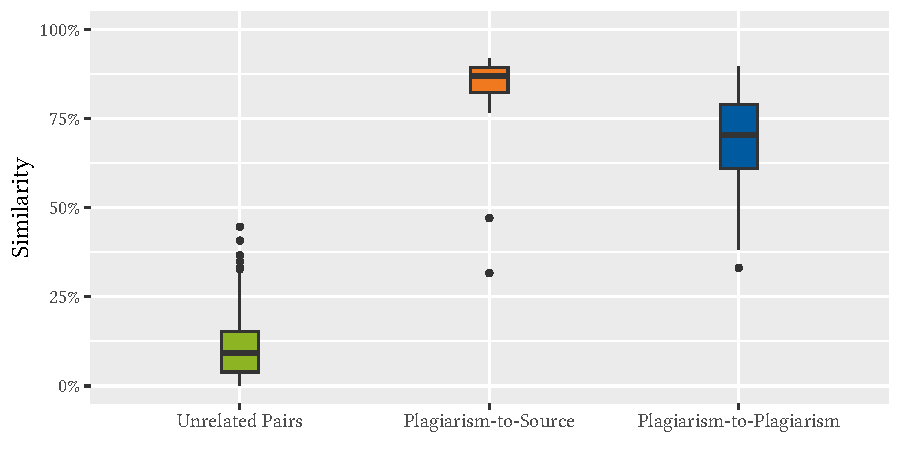
\includegraphics[width=\linewidth]{figures/mde/experiment_avg.similarity.pdf}
    \caption[Detecting Human Obfuscation]{Similarities computed by JPlag for unrelated pairs of original solutions, plagiarism instances with their sources, and plagiarism instances of the same source among each other.}
    \label{fig:jplag-student-obf}
\end{figure} 
    
\begin{table}[H]
		\centering
		\begin{tabular}{l cccccc}
			\toprule
			\textbf{Type}           & \textbf{Median} & \textbf{Mean} & \textbf{Minimum} & \textbf{Maximum} & \textbf{Q1} & \textbf{Q3} \\
			\midrule
			Unrelated\newline Pairs & 14.79        & 15.52         & 0.00         & 51.15        & 10.08       & 20.78       \\
			Plag.-to-Source         & 89.27        & 84.71         & 47.06        & 95.31        & 86.35       & 91.58       \\
			Plag.-to-Plag.          & 77.46        & 72.55         & 42.65        & 92.79        & 64.52       & 85.36       \\
			\bottomrule
		\end{tabular}
		\caption[Detecting Human Obfuscation]{Similarity metrics for the pair types in \autoref{fig:jplag-student-obf}, a higher difference to the unrelated pairs means better detection.}
		\label{tab:jplag-student-obf}
\end{table}

\noindent
To answer whether the plagiarized models can still be detected with a state-of-the-art tool, we employed the token-based plagiarism detector JPlag~\cite{prechelt2002, Saglam2022}.
To create a comprehensive labeled dataset, we combined the plagiarism instances from ten participants, along with their corresponding sources, and included unrelated solutions from previous years. This resulted in a dataset of 31 solutions, which we analyzed using JPlag.
%
JPlag computes similarities for each assignment pair, resulting in 465 pairs, which we depict in \autoref{fig:jplag-student-obf}.
Detecting the relationship between two instances of plagiarism from the same source is significantly more challenging than the relationship between a plagiarism instance and its source; as for the former case, the alterations made by both plagiarizers accumulate, leading to plagiarism up to twice as well obfuscated.
Thus, we separate them into distinct categories, illustrated in \autoref{fig:jplag-student-obf}.

The plagiarism-to-plagiarism pairs exhibit considerably lower similarities, with a median value of 77.5 percent, in contrast to the 89.3 percent for the plagiarism-to-source pairs. Furthermore, except for one outlier, all plagiarism-to-source pairs exhibit higher similarity values than all plagiarism-to-plagiarism pairs.
This outlier is the plagiarism instance by one participant, who achieves the reduced technique with two techniques. First, they were thorough, making 91 individual changes to the source model, corresponding to one change per model element. Second, they heavily relied on reordering model elements, a weakness of JPlag. Nonetheless, the similarity calculated by JPlag is high enough to detect this outlier.
%
Both groups, however, can be clearly distinguished from the pairs of unrelated models, which exhibit a significantly lower median similarity value of 14.8 percent.
In summary, our findings show that modeling plagiarism can be detected automatically.

%\noindent
%\textit{Lessons Learned:}
\subsection{Lessons Learned}
Our experiment revealed that despite the various types of changes, most students predominantly utilized renaming, deletion, and reordering as obfuscation techniques. This highlights the limitations of relying on names for plagiarism detection. In modeling, names hold significant importance compared to code, but they enable effortless obfuscation attacks for plagiarism. Similarly, unique identifiers cannot be solely relied on, as they can be manipulated, hindering the identification of plagiarized elements.
Detection tools should be designed to minimize the impact of easily manipulated characteristics of modeling artifacts.
%
Students rarely utilized type A changes, indicating their intention to refrain from employing overt modifications. They also utilized very few type D changes, which might be more common among experienced modelers.

We observed that the relation between two plagiarism instances of the same original is significantly more challenging to detect than the relations between the plagiarism instances to the original.
Although modeling plagiarism can still be detected by humans or via tools, it may become more challenging with increased time spent obfuscating or with more experienced students.
In our experiment, the instructor often relied on model elements overlooked during the participant's obfuscation attempts, such as \ac{OCL} constraints.
Furthermore, they also noted that manual comparison would be impractical for larger sample sizes, necessitating using a plagiarism detection tool.
The instructor also mentioned that, without a tool, they would not conduct plagiarism checks without an initial suspicion.
These findings emphasize the need for continuous improvement of tool-based detection methods.

%\textit{Limitations:}
\subsection{Threats to Validity}
We now discuss the threats to the validity of our experiment and the measures we took to address them, following standard guidelines in experimental research~\cite{Wohlin2012}.
%
\paragraph{Internal Validity}
Internal validity refers to whether there are influences that can unknowingly affect the analyzed variable concerning causality~\cite{Wohlin2012}.
%
Since this study was conducted in a simulated setting, the plagiarism behavior of the participants might not entirely reflect the complexity or effort of real-life instances. In a controlled environment, the level of effort students apply to conceal plagiarism may be lower than in actual academic settings, which could impact the frequency of the employed changes.
%
Nonetheless, we maintain that these conditions are adequate for observing \textit{how} students plagiarize.
%
\paragraph{External Validity}
External validity concerns the extent to which our findings can be generalized beyond the context of the experiment.
%
Furthermore, motivating students to participate in experiments presents a challenge. To address this, we kept the duration of the experiment relatively short. Nevertheless, the number of participants could be higher. Increasing the number of participants would improve generalizability across diverse educational settings.
%
The experiment used only a single modeling assignment, which may not capture the full range of potential plagiarism strategies. Incorporating assignments of varying complexity or different types, such as behavioral modeling languages (such as sequence diagrams), might reveal additional or unique plagiarism tactics.
%
Similarly, this experiment was limited to a single course conducted in one semester, constraining the variety of educational settings covered. Repeating the study across multiple courses or semesters could improve the generalizability of the results.
%
\paragraph{Construct Validity}
Construct validity refers to the degree to which we measure the theoretical construct we intend to measure.
%
Since the experiment involved only one type of assignment (an \ac{EMF} metamodeling assignment), construct validity may be limited. Including other assignment types, especially those beyond modeling, could help confirm whether the observed plagiarism techniques are specific to modeling or applicable to other domains. Nevertheless, \ac{EMF} widely used in modeling education and metamodeling assignments are typical~\cite{Ciccozzi2018}.
%
\paragraph{Reliability}
Reliability concerns the consistency and replicability of the results.
To ensure reliability, we have made all artifacts of the experiment available in a dedicated reproduction package~\cite{Saglam2023_supp}.
%
\paragraph{Conclusion}
Despite these limitations, the experiment provides valuable insights into techniques students use to plagiarize modeling assignments. These insights contribute to future research and inform the development of plagiarism detection mechanisms tailored to these unique challenges.
